
\section{Contributions from Final State Interactions}

The model uses the virtual nucleon approximation (VNA) to compute inclusive 
observables in electron-induced scattering off the deuteron including the 
effect of final-state interactions.  Amplitudes and observables are computed in 
an unfactorized manner.  This is still work in development.  Current 
calculations include on-shell and off-shell contributions to the FSI 
amplitudes, but the off-shell contribution is calculated neglecting any 
possible singularities of the EM current in the complex plane.  Calculations 
including these are forthcoming.  The inclusive observables are computed using 
the optical theorem in a manner analogous to Ref.~\cite{Cosyn:2013uoa}.  The 
rescattering of the struck nucleon with the spectator is modelled using an 
eikonal amplitude.  Currently, we have chosen to not suppress the off-shell 
contribution to the fsi amplitude in any manner, as to estimate the maximum 
possible effect of FSI.

\begin{figure}[htb]
\begin{center}
  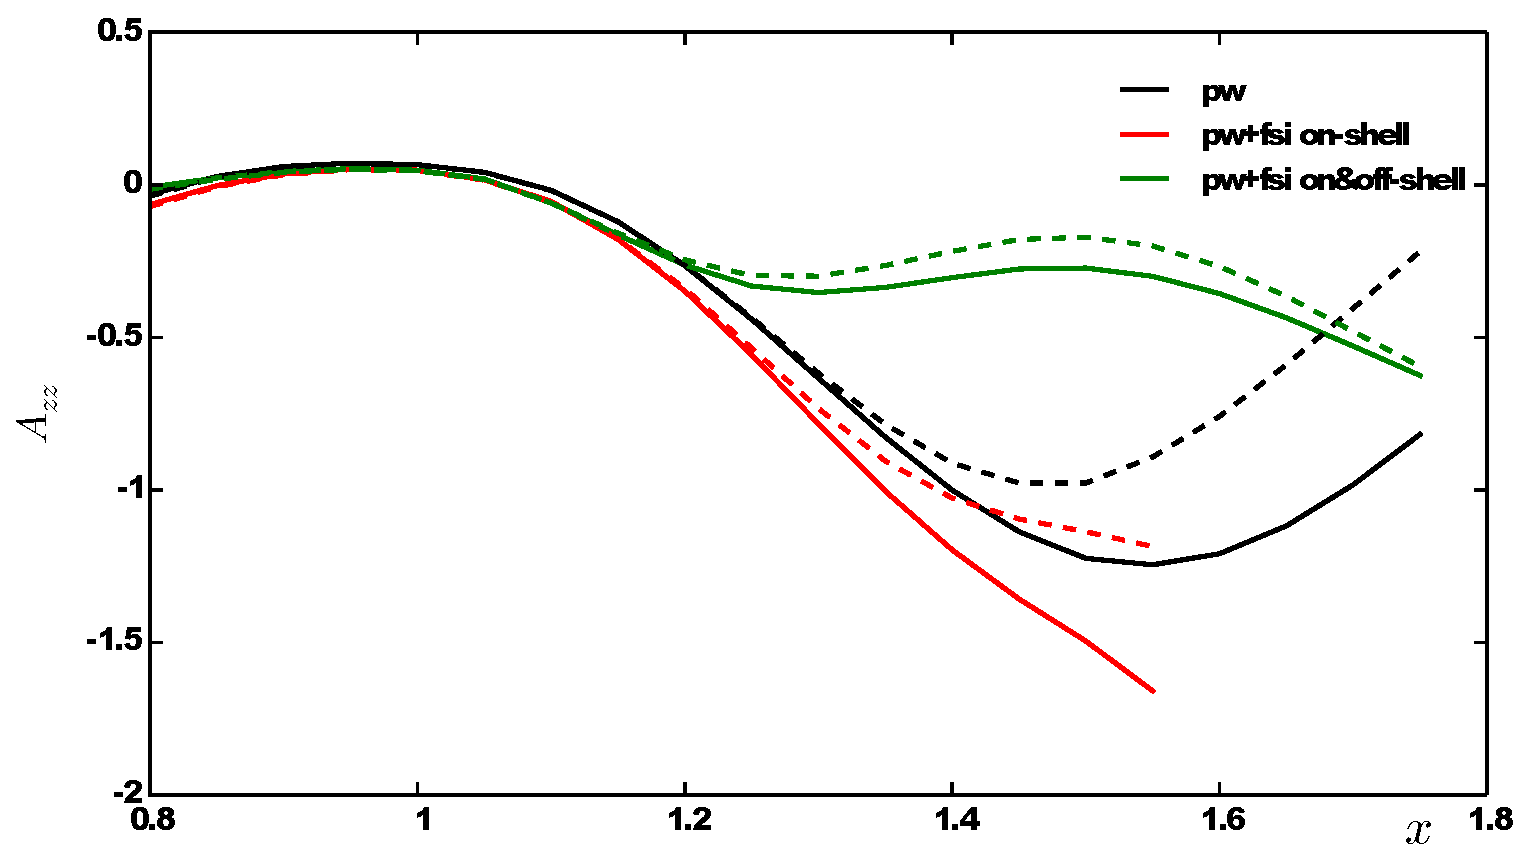
\includegraphics[width=0.5\textwidth]{figs/kin1_cdbonn_av18.eps}
\caption{$A_{zz}$ calculation for kinematic S1 including FSI contributions.  
Full curves use the CDBonn deuteron wave function, dashed ones the AV18 
deuteron wave function.}
\label{fig:kin1}       % Give a unique label
\end{center}
\end{figure}

\begin{figure}[htb]
\begin{center}
  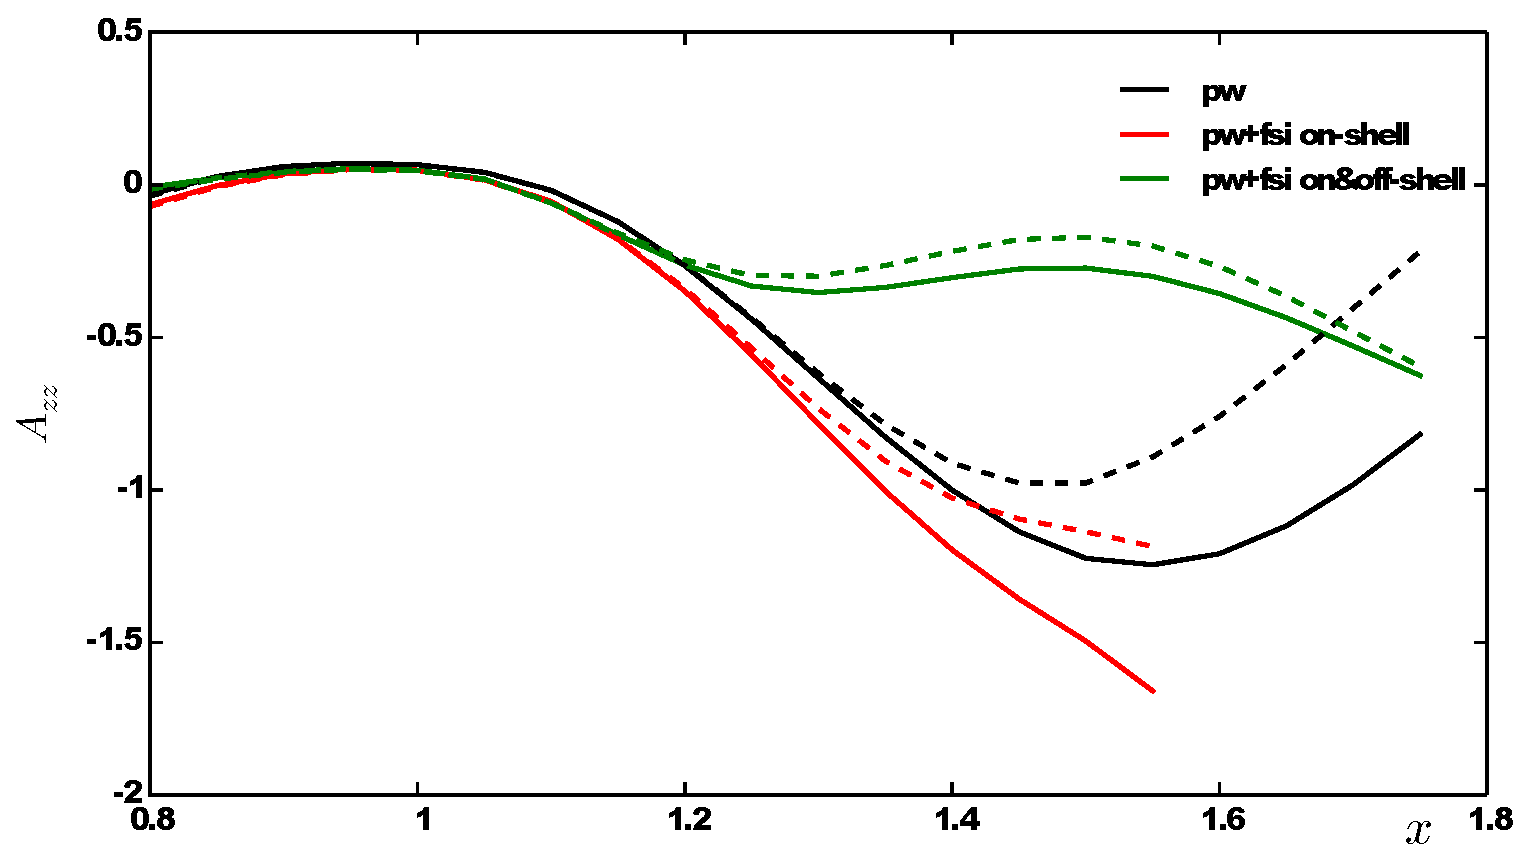
\includegraphics[width=0.5\textwidth]{figs/kin1_cdbonn_av18.eps}
\caption{Same as Fig.~\ref{fig:kin1}, but for kinematic H1}
\label{fig:kin2}       % Give a unique label
\end{center}
\end{figure}

Note: strange bumps in the red curves (plane-wave+on-shell fsi) is due to 
contributions almost cancelling each other in combination with numerical 
errors.  Which means the numerical noise gets enhanced bigtime.  I suggest 
dropping these for now, since the off-shell contribution dominates anyway.

Most theory calculations calculate Azz with a deuteron polarized along the 
virtual photon momentum direction as this limits the number of response 
functions included in the cross section.  For a deuteron polarized along the 
electron beam direction, an extra rotation of the deuteron density matrix needs 
to be accounted for and extra response functions contribute (see Ref. 
\cite{Cosyn:2014sqa} for formulas).  The next figures show how $A_zz$ changes 
when accounting for this.

\begin{figure}[htb]
\begin{center}
  \includegraphics[width=0.5\textwidth]{figs/beampol_av18_kin1.eps}
\caption{$A_{zz}$ calculation for kinematic S1 including FSI contributions 
using the AV18 wave function.  
Full curves use have a deuteron polarized along the photon direction, dashed 
ones along the electron beam.}
\label{fig:beampol1}       % Give a unique label
\end{center}
\end{figure}

\begin{figure}[htb]
\begin{center}
  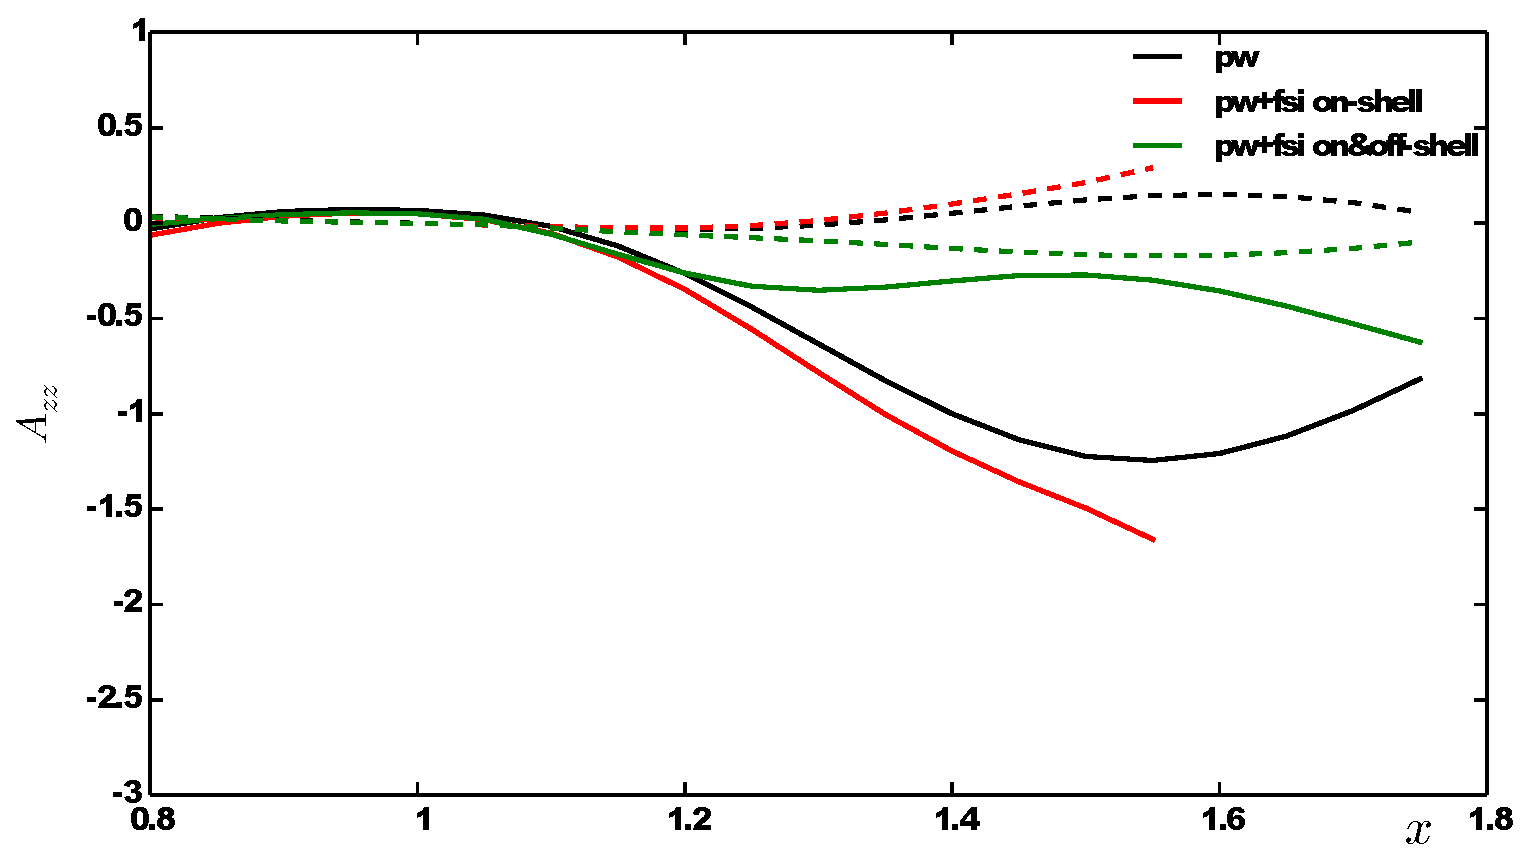
\includegraphics[width=0.5\textwidth]{figs/beampol_cdbonn_kin1.eps}
\caption{Same as Fig.~\ref{fig:beampol1}, but for cdbonn wave function.}
\label{fig:beampol2}       % Give a unique label
\end{center}
\end{figure}

\begin{figure}[htb]
\begin{center}
  \includegraphics[width=0.5\textwidth]{figs/beampol_av18_kin1.eps}
\caption{Same as Fig.~\ref{fig:beampol1}, but H1 kinematics and AV18 wave 
function.}
\label{fig:beampol3}       % Give a unique label
\end{center}
\end{figure}

\begin{figure}[htb]
\begin{center}
  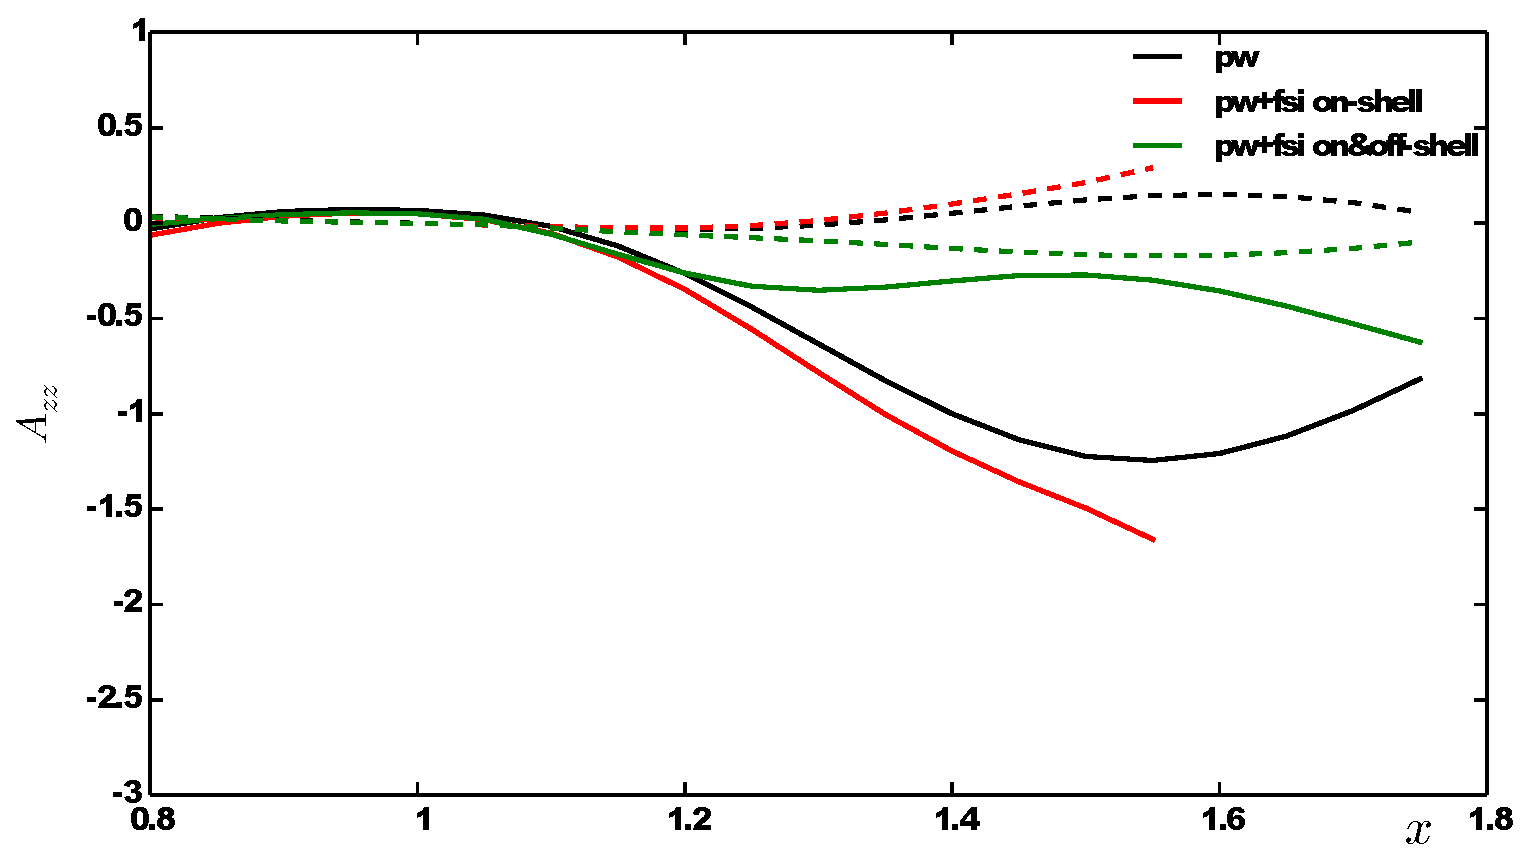
\includegraphics[width=0.5\textwidth]{figs/beampol_cdbonn_kin1.eps}
\caption{Same as Fig.~\ref{fig:beampol1}, but H1 kinematics and cdbonn wave 
function.}
\label{fig:beampol4}       % Give a unique label
\end{center}
\end{figure}


